\documentclass[12pt]{article}

\usepackage{amsmath, amsthm, amssymb}
\usepackage{enumitem}
\usepackage[margin=2.5cm]{geometry}
\usepackage{setspace}
\usepackage{graphicx}
\graphicspath{ {./images/} }

\renewcommand{\baselinestretch}{1.5}
\everymath{\displaystyle}

\begin{document}
	
	\section*{Q1}
	\begin{enumerate}[label=\alph*)]
		\item graphs for mean and standard deviation:\\
		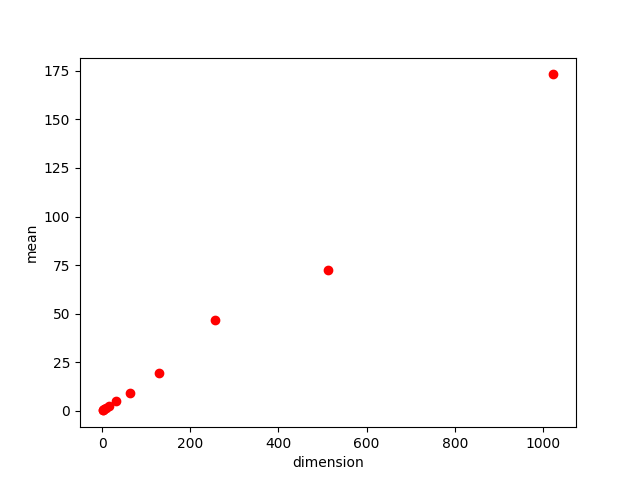
\includegraphics[scale=0.7]{q1a1}\\
		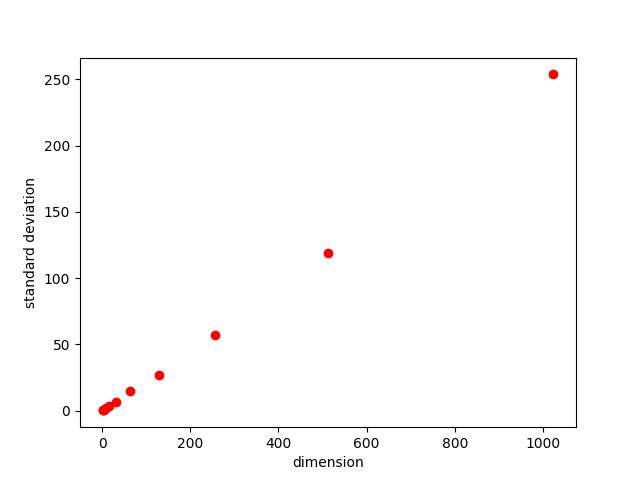
\includegraphics[scale=0.7]{q1a2}
		\item $E[R]=\frac{d}{6}$ and Var$[R]=\frac{7d}{180}$
		\item Markov's Inequality suggests that probability of euclidean distance deviating from expected value very far is unlikely. So that the euclidean distance between two points is likely to be similar (approximately the same distance), and on high dimensions, value of $d$ is large, so $E[R]$ is large. So most points are far away in high dimensions.
	\end{enumerate}

	
	\section*{Q2}
	\begin{enumerate}[label=\alph*)]
		\item see python file
		\item results as followed\\ 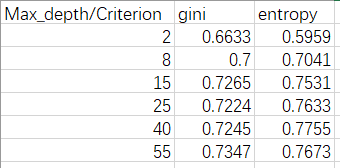
\includegraphics[scale=0.7]{q2b}
		\item tree as followed\\ 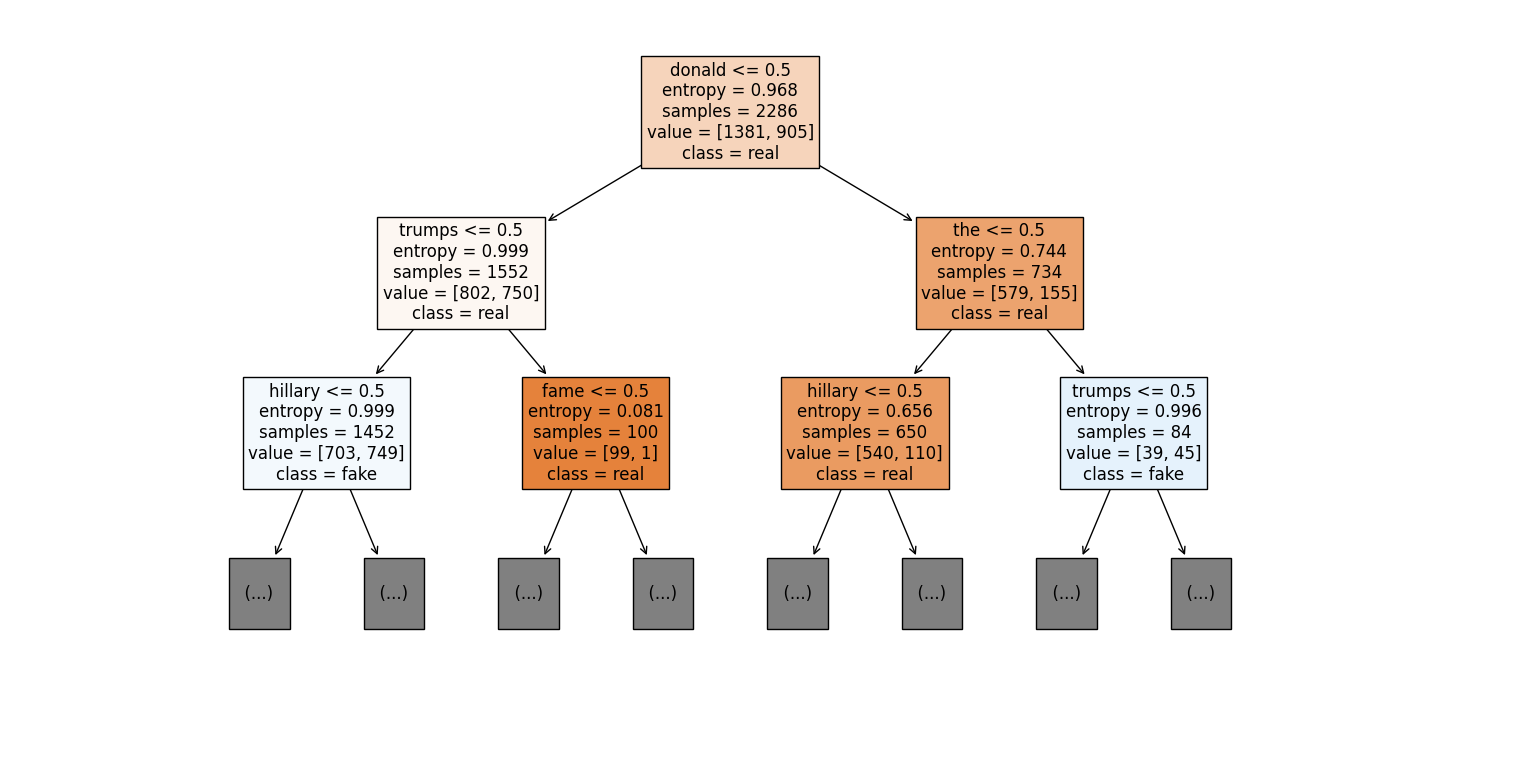
\includegraphics[scale=0.5]{q2c}
		\item At topmost split, the information gain is $0.0513$, with keyword "trump" and class equals real, the information gain is $0.0591$.\\
		With the mutual\_inf\_classif function in sklearn, there is a clear trend of information gain decreasing as we traverse the keyword from the decision tree downwards.
	\end{enumerate}
	
	
	\section*{Q3}
	\begin{enumerate}[label=\alph*)]
		\item Apply definition of gradient descent: 
		\begin{align*}
			w_j &\leftarrow w_j-\alpha\frac{\partial J^\beta_{reg}}{\partial\omega_j}\\
			&=\omega_j-\alpha\cdot(\frac{\partial\mathcal{J}}{\partial\omega_j}+\frac{\partial\mathcal{R}}{\partial\omega_j})\\
			&=\omega_j-\alpha[\frac{1}{2N}\sum^N_{i=1}\frac{\partial}{\partial\omega_j}(y^{(i)}-t^{(i)})^2+\beta_j\omega_j]\\
			&=\omega_j-\alpha[\frac{1}{N}\sum_{i=1}^Nx_j(y^{(i)}-t^{(i)})+\beta_j\omega_j]\\
			&=(1-\alpha\beta_j)\omega_j-\frac{\alpha}{N}\sum_{i=1}^Nx_j(y^{(i)}-t^{(i)})\\
			b &\leftarrow b-\alpha\frac{\partial J^\beta_{reg}}{\partial b}\\
			&=b-\alpha\cdot(\frac{\partial\mathcal{J}}{\partial b}+\frac{\partial\mathcal{R}}{\partial b})\\
			&=b-\alpha[\frac{1}{N}\sum_{i=1}^N(y^{(i)}-x^{(i)})+0]\\
			&=b-\frac{\alpha}{N}\sum_{i=1}^N(y^{(i)}-x^{(i)})
		\end{align*}
		In this method, we adjust the weight in the direction of steepest descent, we multiply $\alpha$ by the weights to prevent it from changing to fast. Therefore the weight is "decaying" to decrease the cost function to minimize the cost function.
		\item Use formula we get from part a)\begin{align*}
			\frac{\partial J^\beta_{reg}}{\partial\omega_j}&=\frac{1}{N}\sum^N_{i=1}x_j^{(i)}(y^{(i)}-t^{(i)})+\beta_j\omega_j\\
			&=\frac{1}{N}\sum_{i=1}^Nx_j^{(i)}(\sum^D_{j'=1}\omega_{j'}x_{j'}^{(i)})-\frac{1}{N}\sum_{i=1}^Nx_j^{(i)}t^{(i)}+\beta_j\omega_j\tag{\text{expand }$y$}\\
			&=\sum_{j'=1}^D\omega_{j'}(\frac{1}{N}\sum_{i=1}^Nx_j^{(i)}x_{j'}^{(i)}+\beta_j(\text{if $\omega_j=\omega_{j'}$}))-\frac{1}{N}\sum_{i=1}^Nx_j^{(i)}t^{(i)}\tag{take out $\omega_{j'}$}\\
			&=\sum_{j'=1}^D\omega_{j'}(\frac{1}{N}\sum_{i=1}^Nx_j^{(i)}x_{j'}^{(i)}+\beta_j\Gamma(\omega_j))-\frac{1}{N}\sum_{i=1}^Nx_j^{(i)}t^{(i)}
		\end{align*} with \begin{equation*}
		\Gamma(\omega_j)=\begin{cases}
			1 \quad j'=j \\ 0 \quad\text{otherwise}
		\end{cases}
	\end{equation*}
		We get $A_{jj'}=\frac{1}{N}\sum_{i=1}^Nx_j^{(i)}x_{j'}^{(i)}+\beta_j\Gamma(\omega_j)$ and $c_j=\frac{1}{N}\sum_{i=1}^Nx_j^{(i)}t^{(i)}$
		\item $\textbf{A}=\frac{1}{N}\textbf{X}^\top\textbf{X}+\lambda D\beta$ where $D$ is the diagonal matrix\\
		$\textbf{c}=\frac{1}{N}\textbf{X}^\top\textbf{t}$\\
		Note we have $\textbf{A}\textbf{w}=\textbf{c}$ from b), expand the equation, we get
		\[(\frac{1}{N}\textbf{X}^\top\textbf{X}+\lambda D\beta)\textbf{w}=\frac{1}{N}\textbf{X}^\top\textbf{t}\]
		Rearrange to get:
		\[\textbf{w}=\textbf{X}^\top\textbf{t}(\textbf{X}^\top\textbf{X}+\lambda ND\beta)^{-1}\]
	\end{enumerate}
	
	
	
	
	
	
	
	
	
	
	
\end{document}